\documentclass[tikz,border=5pt]{standalone}
\usepackage{amsmath,amssymb}
\usetikzlibrary{arrows.meta,calc,decorations.markings,patterns,positioning}

\definecolor{active}{RGB}{176,43,43}
\definecolor{inactive}{RGB}{39,100,155}
\definecolor{surface}{RGB}{242,236,214}
\definecolor{section}{RGB}{90,90,90}
\definecolor{cuff}{RGB}{38,38,38}

\tikzset{
  panel/.style={draw=black!35, rounded corners=2pt, line width=.35pt},
  surf/.style={draw=black!75, fill=surface, line width=.65pt},
  cuff/.style={draw=cuff, line width=.9pt},
  active/.style={draw=active, line width=1.05pt},
  inactive/.style={draw=inactive, fill=inactive!18, line width=.8pt},
  section/.style={draw=section, densely dotted, line width=.8pt},
  every node/.style={font=\footnotesize, inner sep=1.5pt},
  >=Latex
}

\begin{document}
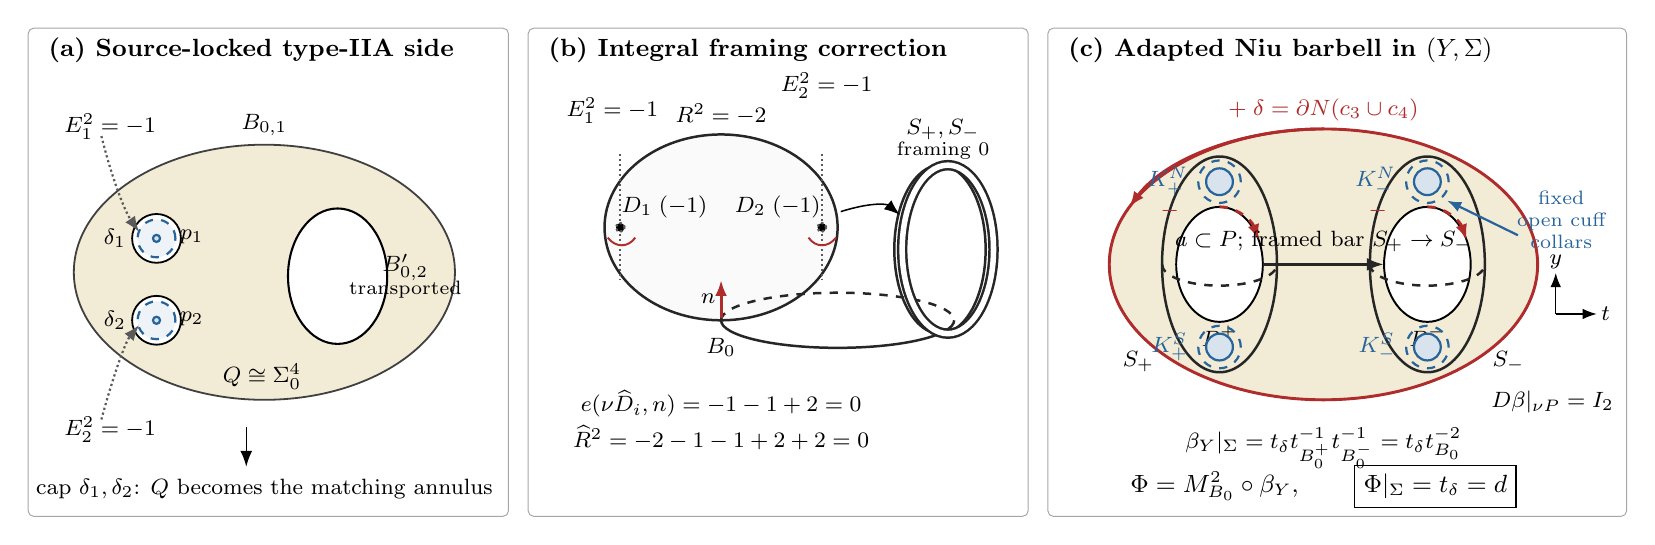
\begin{tikzpicture}[x=1cm,y=1cm]

% ------------------------------------------------------------------
% Panel A: four-holed source region
% ------------------------------------------------------------------
\begin{scope}[shift={(0,0)}]
  \draw[panel] (-.35,-3.05) rectangle (5.75,3.15);
  \node[anchor=west,font=\bfseries\small] at (-.15,2.87)
    {(a) Source-locked type-IIA side};

  \draw[surf] (2.65,0.05) ellipse (2.42 and 1.62);
  \node at (2.62,-1.28) {$Q\cong\Sigma_0^4$};
  \node[anchor=south] at (2.65,1.72) {$B_{0,1}$};

  % three interior holes: two capped boundary components and transported B0
  \draw[fill=white,line width=.65pt] (1.28,.48) circle (.31);
  \draw[fill=white,line width=.65pt] (1.28,-.56) circle (.31);
  \draw[fill=white,line width=.75pt] (3.58,0) ellipse (.63 and .86);
  \node[left] at (.95,.48) {$\delta_1$};
  \node[left] at (.95,-.56) {$\delta_2$};
  \node[align=center] at (4.44,0)
    {$B'_{0,2}$\\[-1pt]\scriptsize transported};

  % cap disks and section centers
  \draw[inactive,dashed,fill=inactive!8] (1.28,.48) circle (.24);
  \draw[inactive,dashed,fill=inactive!8] (1.28,-.56) circle (.24);
  \fill[inactive] (1.28,.48) circle (.045);
  \fill[inactive] (1.28,-.56) circle (.045);
  \node[right] at (1.52,.50) {$p_1$};
  \node[right] at (1.52,-.54) {$p_2$};

  \draw[section,-{Latex[length=2mm]}] (.58,1.78)
    .. controls (.72,1.22) and (.88,.82) .. (1.06,.56);
  \draw[section,-{Latex[length=2mm]}] (.58,-1.82)
    .. controls (.72,-1.30) and (.88,-.84) .. (1.06,-.62);
  \node[anchor=west] at (.05,1.90) {$E_1^2=-1$};
  \node[anchor=west] at (.05,-1.95) {$E_2^2=-1$};

  \draw[-{Latex[length=2mm]},line width=.55pt]
    (2.42,-1.92) -- (2.42,-2.42);
  \node[align=center] at (2.65,-2.70)
    {cap $\delta_1,\delta_2$: $Q$ becomes the matching annulus};
\end{scope}

% ------------------------------------------------------------------
% Panel B: section resolution and framing
% ------------------------------------------------------------------
\begin{scope}[shift={(6.25,0)}]
  \draw[panel] (-.25,-3.05) rectangle (6.10,3.15);
  \node[anchor=west,font=\bfseries\small] at (-.05,2.87)
    {(b) Integral framing correction};

  % original matching sphere split into two disks
  \draw[cuff,fill=black!2] (2.20,.62) ellipse (1.48 and 1.18);
  \draw[cuff] (2.20,-.56) arc[start angle=180,end angle=360,
                                   x radius=1.48,y radius=.35];
  \draw[cuff,dashed] (2.20,-.56) arc[start angle=180,end angle=0,
                                      x radius=1.48,y radius=.35];
  \node[above] at (2.20,1.86) {$R^2=-2$};
  \node at (1.48,.88) {$D_1\;(-1)$};
  \node at (2.92,.88) {$D_2\;(-1)$};
  \node[below] at (2.20,-.73) {$B_0$};

  % prescribed equatorial normal
  \draw[active,-{Latex[length=2mm]}] (2.20,-.53) -- (2.20,-.05)
    node[midway,left,text=black] {$n$};

  % section intersections and resolution bands
  \draw[section] (.92,1.55) -- (.92,-.05);
  \draw[section] (3.48,1.55) -- (3.48,-.05);
  \fill[section] (.92,.62) circle (.055);
  \fill[section] (3.48,.62) circle (.055);
  \node[anchor=west] at (.18,2.10) {$E_1^2=-1$};
  \node[anchor=east] at (4.18,2.42) {$E_2^2=-1$};
  \draw[active,line width=.7pt] (.76,.49) .. controls (.86,.36) and
                                      (1.02,.36) .. (1.11,.49);
  \draw[active,line width=.7pt] (3.31,.49) .. controls (3.40,.36) and
                                      (3.56,.36) .. (3.66,.49);

  \node[align=center] at (2.20,-1.62)
    {$e(\nu\widehat D_i,n)=-1-1+2=0$};
  \node[align=center] at (2.20,-2.05)
    {$\widehat R^2=-2-1-1+2+2=0$};

  % two parallel cuffs after completion
  \draw[cuff] (4.98,.34) ellipse (.58 and 1.07);
  \draw[cuff,double distance=2pt] (5.08,.34) ellipse (.58 and 1.07);
  \node[align=center] at (5.02,1.74)
    {$S_+,S_-$\\[-2pt]\scriptsize framing $0$};
  \draw[-{Latex[length=2mm]},line width=.55pt] (3.72,.82)
    .. controls (4.10,.94) and (4.30,.92) .. (4.47,.78);
\end{scope}

% ------------------------------------------------------------------
% Panel C: adapted barbell and active/inactive pieces
% ------------------------------------------------------------------
\begin{scope}[shift={(12.85,0)}]
  \draw[panel] (-.25,-3.05) rectangle (7.10,3.15);
  \node[anchor=west,font=\bfseries\small] at (-.05,2.87)
    {(c) Adapted Niu barbell in $(Y,\Sigma)$};

  % pair of pants as an oval with two holes
  \draw[surf] (3.25,.15) ellipse (2.72 and 1.72);
  \draw[fill=white,line width=.7pt] (1.93,.15) ellipse (.55 and .73);
  \draw[fill=white,line width=.7pt] (4.57,.15) ellipse (.55 and .73);

  % outer boundary delta and active positive twist
  \draw[active] (3.25,.15) ellipse (2.72 and 1.72);
  \draw[active,-{Latex[length=2mm]}]
    (3.25,1.87) arc[start angle=90,end angle=155,
                     x radius=2.72,y radius=1.72];
  \node[text=active,anchor=south] at (3.25,1.91)
    {$+\;\delta=\partial N(c_3\cup c_4)$};

  % cuffs shown as vertical spheres through inner boundaries
  \draw[cuff] (1.93,.15) ellipse (.73 and 1.37);
  \draw[cuff] (4.57,.15) ellipse (.73 and 1.37);
  \draw[cuff,dashed] (1.20,.15) arc[start angle=180,end angle=360,
                                       x radius=.73,y radius=.27];
  \draw[cuff,dashed] (3.84,.15) arc[start angle=180,end angle=360,
                                       x radius=.73,y radius=.27];
  \node[anchor=east] at (1.16,-1.08) {$S_+$};
  \node[anchor=west] at (5.34,-1.08) {$S_-$};
  \node[below] at (1.93,-.57) {$B_0^+$};
  \node[below] at (4.57,-.57) {$B_0^-$};

  % inner negative active twists
  \draw[active,dashed,-{Latex[length=2mm]}]
    (1.93,.88) arc[start angle=90,end angle=25,x radius=.55,y radius=.73];
  \draw[active,dashed,-{Latex[length=2mm]}]
    (4.57,.88) arc[start angle=90,end angle=25,x radius=.55,y radius=.73];
  \node[text=active] at (1.30,.83) {$-$};
  \node[text=active] at (3.94,.83) {$-$};

  % bar in P
  \draw[cuff,line width=1.25pt,-{Latex[length=2.2mm]}]
    (2.48,.15) -- (4.02,.15);
  \node[above,align=center] at (3.25,.25)
    {$a\subset P$; framed bar $S_+\to S_-$};

  % four inactive disk germs with halos
  \foreach \x in {1.93,4.57} {
    \draw[inactive] (\x,1.20) circle (.17);
    \draw[inactive,dashed,fill=none] (\x,1.20) circle (.27);
  }
  \foreach \x in {1.93,4.57} {
    \draw[inactive] (\x,-.90) circle (.17);
    \draw[inactive,dashed,fill=none] (\x,-.90) circle (.27);
  }
  \node[text=inactive,anchor=east] at (1.59,1.20) {$K_+^N$};
  \node[text=inactive,anchor=east] at (4.23,1.20) {$K_-^N$};
  \node[text=inactive,anchor=east] at (1.59,-.90) {$K_+^S$};
  \node[text=inactive,anchor=east] at (4.23,-.90) {$K_-^S$};
  \node[text=inactive,align=center,text width=1.25cm,font=\scriptsize]
    at (6.27,.72) {fixed open cuff collars};
  \draw[inactive,-{Latex[length=1.8mm]}] (5.72,.52) -- (4.82,.96);

  % normal coordinates
  \coordinate (O) at (6.20,-.48);
  \draw[-{Latex[length=1.8mm]}] (O) -- ++(.52,0) node[right] {$t$};
  \draw[-{Latex[length=1.8mm]}] (O) -- ++(0,.52) node[above] {$y$};
  \node[align=center] at (6.16,-1.60)
    {$D\beta|_{\nu P}=I_2$};

  \node[align=center] at (3.25,-2.18)
    {$\beta_Y|_\Sigma=t_\delta t_{B_0^+}^{-1}t_{B_0^-}^{-1}
      =t_\delta t_{B_0}^{-2}$};
  \node[align=center,font=\small] at (3.25,-2.67)
    {$\Phi=M_{B_0}^{2}\circ\beta_Y,\qquad
      \boxed{\Phi|_\Sigma=t_\delta=d}$};
\end{scope}

\end{tikzpicture}
\end{document}
